\state{Some one-dimensional chemistry}{
	Consider a diatomic lattice of two atoms labeled $A$ and $B$ in a lattice with period $a$, at the positions $\pm a (1 - \del) / 4$ in a one-dimensional array with overall period $a$.
}

\prob{	\label{5a}
	Using the NFE approximation valid for momenta near the zone boundary $k \to \pi / a$, show that the solution of Eq.~(4.47) leads to 
	\begin{enumerate}
		\item a gap on the zone boundary of $2 \abs{ \Utpa }$, and
		\item wavefunctions that satisfy $\cpmk / \cpmkmpa = \pm U / \abs{U}$ as $k \to \pi / a$.
	\end{enumerate}
}

\sol{
	Equation~(4.47) is
	\eq{
		\mqty( \Eok - E & \UvK \\ \UvKs & \EokmK - E ) \mqty( \ck \\ \ckmK ) = 0.
	}
	According to p.~43 of the lecture notes, the Brillouin zone boundary is at $\vK / 2$, so $\vK = 2\pi / a$.  Then Eq.~(4.47) is
	\eq{
		\mqty( \Eok - E & \Utpa \\ \Utpas & \Eokmtpa - E ) \mqty( \ck \\ \ckmK ) = 0
	}
	which implies that the determinant of the $2 \times 2$ matrix is 0~\cite[p.~158]{Ashcroft}:
	\al{
		0 &= \mqty| \Eok - E & \Utpa \\ \Utpas & \Eokmtpa - E | \\
		&= (\Eok - E) (\Eokmtpa - E) - \abs{\Utpa}^2 \\
		&= E^2 - (\Eok + \Eokmtpa) E + \Eok \Eokmtpa - \abs{\Utpa}^2.
	}
	Solving for $E$ using the quadratic equation yields
	\eq{
		\Epm = \frac{\Eok + \Eokmtpa}{2} \pm \sqrt{ \paren{\frac{\Eok - \Eokmtpa}{2}}^2 + \abs{\Utpa}^2 }.
	}
	Applying $\Eok = \hbar^2 k^2 / 2m$ from p.~42 of the lecture notes, this is
	\eqn{Epm}{
		\Epm = \frac{\hbar^2}{4m} \brac{ k^2 + \paren{ k - \frac{2\pi}{a} }^2 } \pm \sqrt{ \paren{ \frac{\hbar^2}{4m} }^2 \brac{ k^2 - \paren{ k - \frac{2\pi}{a} }^2 }^2 + \abs{\Utpa}^2 }.
	}
	At the zone boundary $k = \pi / a$, and
	\al{
		\Epm &= \frac{\hbar^2}{4m} \brac{ \paren{ \frac{\pi}{a} }^2 + \paren{ \frac{\pi}{a} - \frac{2\pi}{a} }^2 } \pm \sqrt{ \paren{ \frac{\hbar^2}{4m} }^2 \brac{ \paren{ \frac{\pi}{a} }^2 - \paren{ \frac{\pi}{a} - \frac{2\pi}{a} }^2 }^2 + \abs{\Utpa}^2 } \\
		&= \frac{\hbar^2}{4m} \paren{ 2 \frac{\pi^2}{a^2} } \pm \sqrt{ \abs{\Utpa}^2 } \\
		&= \frac{\hbar^2}{2m} \frac{\pi^2}{a^2} \pm \abs{\Utpa}.
	}
	Then the gap is
	\eq{
		\Ep - \Em = \paren{ \frac{\hbar^2}{2m} \frac{\pi^2}{a^2} + \abs{\Utpa} } - \paren{ \frac{\hbar^2}{2m} \frac{\pi^2}{a^2} - \abs{\Utpa} }
		= \ans{ 2 \abs{\Utpa} }
	}
	as we wanted to show. \qed

	
	At $k = \pi / a = K / 2$, the energy levels are given by (4.49) in the lecture notes,
	\eqn{4.49}{
		\Epm(K / 2) = \EohK \pm \abs{\UK}.
	}
	The leading corrections in $U$ for two energy levels are given by Ashcroft \& Mermin~(9.22),
	\al{
		(E - \Eok) \ck &= \UvK \ckmK, &
		(E - \EokmK) \ckmK &= \UmvK \ck
		= \UvKs \ck,
	}
	where $\ck$ and $\ckmK$ are the coefficients of the wavefunctions.  Substituting $k = \pi / a$ and $K = 2\pi / a$ and Eq.~\refeq{4.49} into the first of these expressions, we find
	\eq{
		\Utpa \cpmkmpa = (\Epm - \Eopa) \cpmk
		= [ (\Eopa \pm \abs{\Utpa}) - \Eopa ] \cpmk
		= \pm \abs{\Utpa} \cpmk
	}
	which implies
	\eqn{ratio}{
		\ans{ \frac{\cpmk}{\cpmkmpa} = \pm \frac{\Utpa}{\abs{\Utpa}} }
	}
	as desired~\cite[p.~159]{Ashcroft}. \qed
	
}



\prob{
	Hence show that the probability density for the electronic states at $k = \pi / a$ take the form
	\aln{ \label{densities}
		\abs{\psipr}^2 &\propto \cos[2](\frac{\pi x}{a} + \frac{\phi}{2}), &
		\abs{\psimr}^2 &\propto \sin[2](\frac{\pi x}{a} + \frac{\phi}{2}).
	}
}

\sol{
	The wavefunctions are given by (4.38) in the lecture notes,
	\eq{
		\psivkr = \sumK \ckmK e^{i (\vk - \vK) \vdot \vr}.
	}
	With $k = \pi / a$, this gives us
	\al{
		\psipr &= \cpk e^{i k x} + \cpkmpa e^{i (k - 2\pi / a) x}
		= \cpk (e^{i \pi x / a} + e^{-i \pi x / a})
		= 2 \cpk \cos(\frac{\pi x}{a}), \\
		\psimr &= \cmk e^{i k x} - \cmkmpa e^{i (k - 2\pi /a) x}
		= \cmk (e^{i \pi x / a} - e^{-i \pi x / a})
		= 2 i \cmk \sin(\frac{\pi x}{a}),
	}
	where we have used Eq.~\refeq{ratio}.  Then
	\al{
		\abs{\psipr}^2 &= -2 \abs{\cpk}^2 \cos[2](\frac{\pi x}{a})
		\propto \ans{ \cos[2](\frac{\pi x}{a} + \frac{\phi}{2}), } \\
		\abs{\psimr}^2 &= 2 \abs{\cmk}^2 \sin[2](\frac{\pi x}{a})
		\propto \ans{ \sin[2](\frac{\pi x}{a} + \frac{\phi}{2}), }
	}
	where we have included a phase shift $\phi / 2$ in order to account for the complex coefficient. \qed
}



\prob{
	Show that the potential can be written
	\eqn{Utpa}{
		\Utpa = \sin(\frac{\pi \del}{2}) \paren{ \UAtpa + \UBtpa } - i \cos(\frac{\pi \del}{2}) \paren{ \UAtpa - \UBtpa },
	}
	where
	\eq{
		\UABtpa = \frac{N}{V} \int \ddr e^{-2 \pi i r / a} \UABr.
	}
}

\sol{
	Since $\Ur$ is a sum of atomic potentials located at the positions of the atoms, it can be written as Ashcroft \& Mermin~(9.31):
	\aln{
		\Ur &= \sumvR \brac{ \UA(\vr - \vR - \vdA) + \UB(\vr - \vR - \vdB) } \notag \\
		&= \sumvR \brac{ \UA\!\paren{ \vr - \vR - \frac{a}{4} (1 - \del) } + \UB\!\paren{ \vr - \vR + \frac{a}{4} (1 - \del) } }, \label{thing5c}
	}
	where $\vdA$ and $\vdB$ are the positions of the atoms.  The momentum components of the potential are given by (4.20) in the lecture notes:
	\eq{
		\UvG = \frac{N}{V} \intuc \ddvr e^{-i \vG \vdot \vr} \Uvr.
	}
	Feeding in Eq.~\refeq{thing5c} and $K = 2 \pi / a$,
	\al{
		\UK &= \frac{N}{V} \intuc \ddr e^{-i K r} \sumR \brac{ \UA\!\paren{ r - R - \frac{a}{4} (1 - \del) } + \UB\!\paren{ r - R + \frac{a}{4} (1 - \del) } } \\
		&= \frac{N}{V} \brac{ \intas \ddr e^{-i K r} \UA\!\paren{ r - \frac{a}{4} (1 - \del) } + \intas \ddr e^{-i K r} \UB\!\paren{ r  + \frac{a}{4} (1 - \del) } }.
	}
	Let $r' = r \mp a (1 - \del) / 4$.  Then
	\eq{
		\UK = \frac{N}{V} \intas \ddrp e^{-i K r'} \brac{ e^{-i K a (1 - \del) / 4} \UArp + e^{-i K a (1 + \del) / 4} \UBrp }.
	}
	Renaming $r' \to r$ and applying $K = 2\pi / a$, we have
	\al{
		\Utpa &= \frac{N}{V} \intas \ddr e^{-i 2\pi r / a} \brac{ e^{-i 2\pi (1 - \del) / 4} \UAr + e^{-i 2\pi (1 + \del) / 4} \UBr } \\
		&= e^{-i \pi / 2} \frac{N}{V} \intas \ddr e^{-i 2\pi r / a} \brac{ e^{i \pi \del / 2} \UAr - e^{-i \pi \del / 2} \UBr } \\
		&= i \frac{N}{V} \brac{ \int \ddr e^{-i \pi (2 r / a + \del / 2)} \UBr - \int \ddr e^{-i \pi (2 r / a - \del / 2)} \UAr } \\
		&= i \frac{N}{V} \brac{ e^{-i \pi \del / 2} \int \ddr e^{-2 \pi i r / a} \UBr - e^{i \pi \del / 2} \int \ddr e^{-2 \pi i r / a} \UAr } \\
		&= i \brac{ e^{-i \pi \del / 2} \UBtpa - e^{i \pi \del / 2} \UAtpa } \\
		&= \frac{i}{2} \brac{ e^{-i \pi \del / 2} (\UAtpa + \UBtpa - \UAtpa + \UBtpa) - e^{i \pi \del / 2} (\UAtpa + \UBtpa + \UAtpa - \UBtpa) } \\
		&= \frac{i}{2} (e^{-i \pi \del / 2} - e^{i \pi \del / 2}) \paren{ \UAtpa + \UBtpa } - \frac{i}{2} (e^{-i \pi \del / 2} + e^{i \pi \del / 2}) \paren{ \UAtpa - \UBtpa } \\
		&= \ans{ \sin(\frac{\pi \del}{2}) \paren{ \UAtpa + \UBtpa } - i \cos(\frac{\pi \del}{2}) \paren{ \UAtpa - \UBtpa } }
	}
	as we wanted to show. \qed
}



\prob{
	The system contains an average of one electron per atom, or equivalently two electrons per unit cell.  Discuss the values of the energy gaps and plot the charge densities corresponding to the highest filled electron state and the lowest empty electron state in the two cases:
	\begin{enumerate}
		\item $\del = 0$, $\UsA \neq \UsB$;
		\item identical atoms, $\UsA = \UsB$, and $\del \neq 0$.
	\end{enumerate}
	Explain how this provides a simple model of either an \emph{ionic} or \emph{covalent} solid.
}

\sol{
	We know that the energy gap is $2 \abs{\Utpa}$.  In the first case, substituting $\del = 0$ into Eq.~\refeq{Utpa} gives us
	\eq{
		\Utpa = \sin(0) \paren{ \UAtpa + \UBtpa } - i \cos(0) \paren{ \UAtpa - \UBtpa }
		= -i \paren{ \UAtpa - \UBtpa }
	}
	so the energy gap is
	\eq{
		2 \abs{\Utpa} = \ans{ 2 \abs{ \UAtpa - \UBtpa }. }
	}
	The charge density corresponding to the highest filled electron state is $\abs{\psimr}^2$, and that corresponding to the lowest empty electron state is $\abs{\psipr}^2$.  When $\del = 0$, the atoms are uniformly spaced so $\phi = n \pi / 2$ with $n$ an odd integer.  Figure~\refeq{5d}~(top) shows the positions of the atoms $A$ and $B$ as well as $\abs{\psipmr}^2$ from Eq.~\refeq{densities}.  The $A$ atoms (red dots) have positions $a (1 - \del) / 4$, and the $B$ atoms (violet dots) have positions $-a (1 - \del) / 4$.  In the figure $\abs{\psimr}^2$ is shown by a dotted gold line and $\abs{\psipr}^2$ by a dotted blue line.  The charge densities show that the electron in a particular state is localized near one atom.  This is representative of an \ans{\emph{ionic}} solid, which has one electron ``donated'' to the more positive ion.
	
	\fig{5d}{
		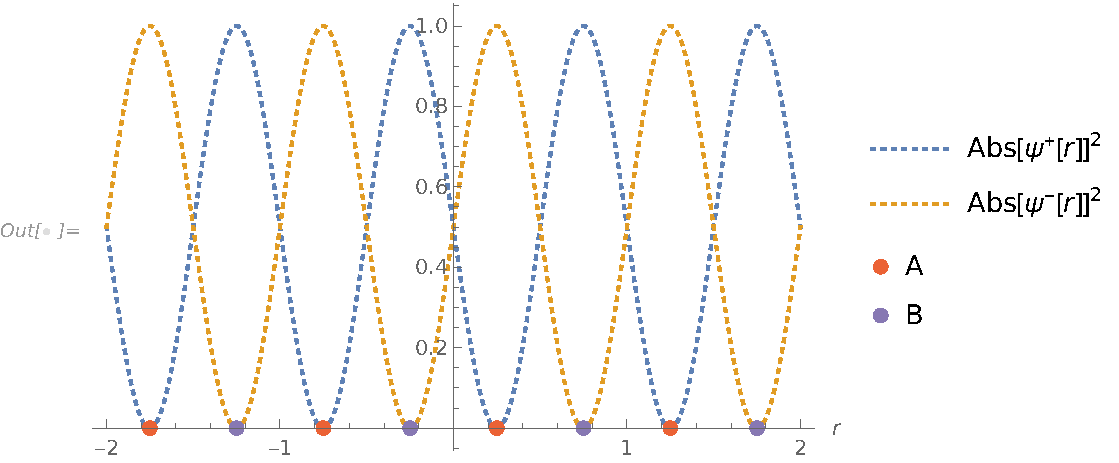
\includegraphics[width=0.6\textwidth,trim=1.4cm 0 0 0,clip]{5di} \\
		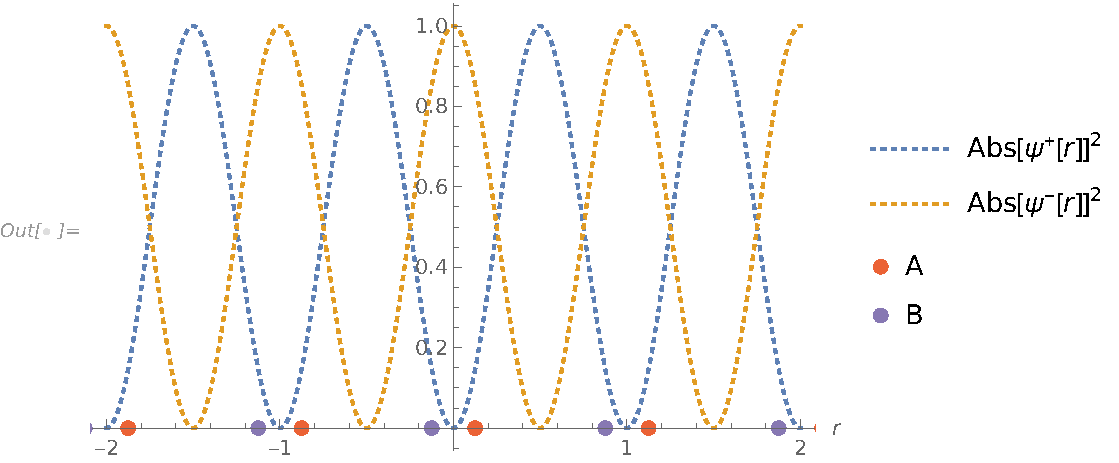
\includegraphics[width=0.6\textwidth,trim=1.4cm 0 0 0,clip]{5dii}
		\caption{Plot of charge densities for the highest filled electron state, $\abs{\psimr}^2$~(gold dotted line), and the lowest empty electron state~(blue dotted line), $\abs{\psipr}^2$, along with $A$ atoms~(red dots) and $B$ atoms~(violet dots).  The charge densities are given by Eq.~\refeq{densities} with (top) $\del = 0$, $\UsA \neq \UsB$, $\phi = n \pi / 2$ for $n$ odd; and with (bottom) $\del = 1/8$, $\UsA = \UsB$, $\phi = n \pi / 2$ for $n$ even.  The top~(bottom) panel demonstrates an ionic~(a covalent) solid.}
	}
	
	In the second case, substituting $\UsA = \UsB$ into Eq.~\refeq{Utpa} yields
	\eq{
		\Utpa = \sin(\frac{\pi \del}{2}) \paren{ \UAtpa + \UAtpa } - i \cos(\frac{\pi \del}{2}) \paren{ \UAtpa - \UAtpa }
		= 2 \sin(\frac{\pi \del}{2}) \UAtpa,
	}
	so the energy gap is
	\eq{
		2 \abs{\Utpa} = \ans{ 4 \abs{ \sin(\frac{\pi \del}{2}) \UAtpa }. }
	}
	When $\del \neq 0$, the atoms are not uniformly spaced so $\phi = n \pi / 2$ with $n$ an even integer.  The charge densities for this scenario are shown in Fig.~\refeq{5d}~(bottom), with $\del = 1/8$.  Here the charge densities show that the electron in a particular state is localized between the ions.  This is a model of a \ans{\emph{covalent}} solid, which has one or more electrons ``shared'' between ions of similar charge.
}